%%%%%%%%%%%%%%%%%%%%%%%%%
\section{\applicationName} \label{projectDesign}
%%%%%%%%%%%%%%%%%%%%%%%%%
The upcoming sections will illustrate \applicationName\ features and how they were developed. The first part proposes the \applicationName\ modelling of data. Afterwards we present a section about the parser and the cron--jobs created. It follows a description of the API provided to the user. Finally this chapter concludes with some discussions about how we developed the structure and the logic behind the Web--Application.

\subsection{\applicationName\ Architecture and Technologies}
The environments selected to develop \applicationName\ are the following:
\begin{itemize}
	\item {\bf The Server--side} was written using the {\bf Java} Programming Language. The {\bf Spring Framework} was used, in particular using its most famous convention--over--configuration, called {\bf Spring Boot}. The database used to store the information about the city is {\bf MySQL}.
	\item {\bf The Client--side} was written using the {\bf Javascript} scripting language. The {\bf jQuery} library was used and, of course, {\bf HTML5} and {\bf CSS3}. As mentioned above, the 3D visualization of the city was achieved using the {\bf Cesium Framework}
\end{itemize}
Figure \ref{fig:project_structure} shows the structure of the final \applicationName\ 's prototype.
\begin{figure}[H]
\centering
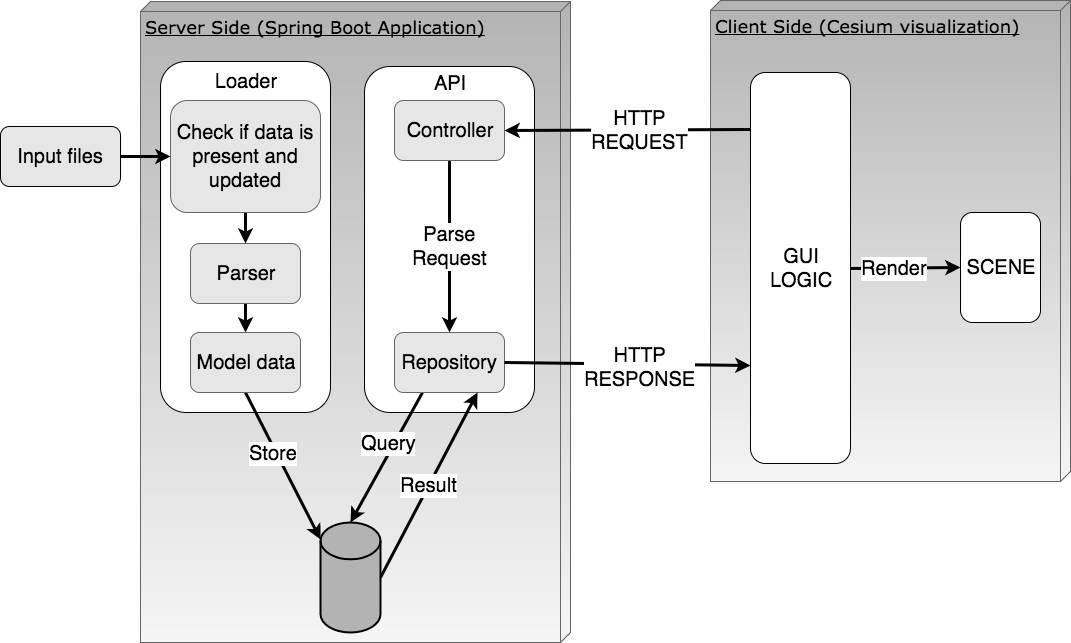
\includegraphics[width=1.0\textwidth]{chapter3/images/project_structure}
\caption{\applicationName\ architecture scheme}
\label{fig:project_structure}
\end{figure}

\subsection{Server Side}
\subsubsection{Available Data and Modelling}
The entire work starts from the ``xml'' file provided by the Comune of Lugano. The first choice to take was how to model the available data in the best way such that the way of retrieving information about any building was as fast and as consistent as possible.\\
The models created are the following: City, Suburb, Building, Address and Type. Figure \ref{fig:db_structure} shows, in the form of an ER diagram, the final version of how the data was modelled into the database, specifying columns and relations between tables.
\begin{figure}[H]
\centering
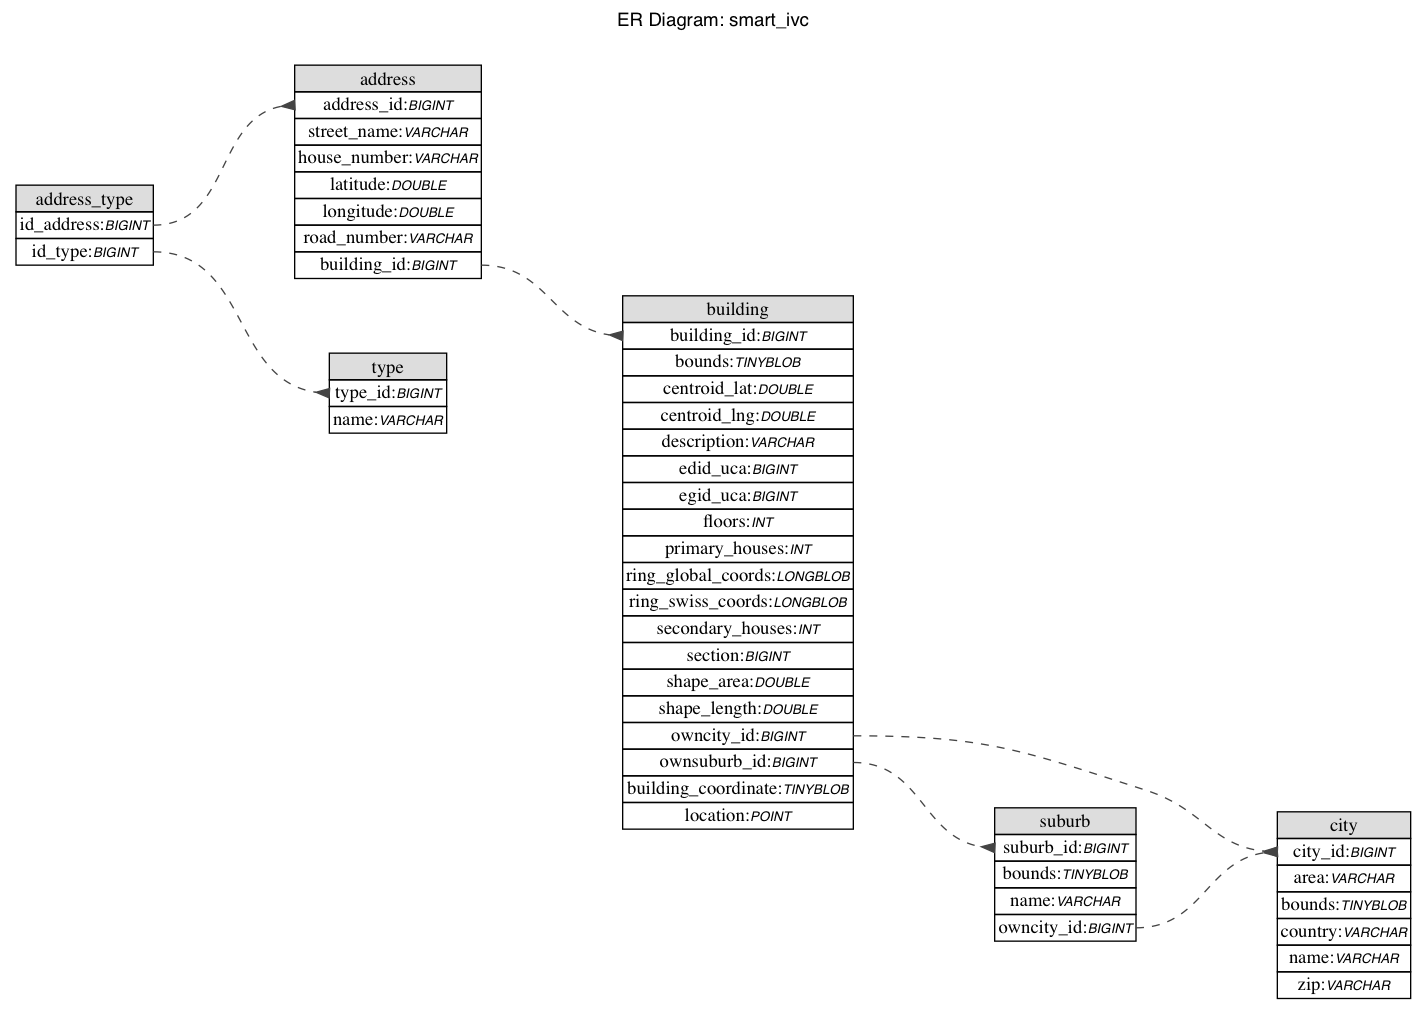
\includegraphics[width=0.8\textwidth]{chapter3/images/db_structure}
\caption{\applicationName\ database structure}
\label{fig:db_structure}
\end{figure}
\subsubsection{Parser}
The data type taken as input is of xml type. It is used in the process to load buildings data.\\
The beginning of the file contains an header which describes the schema of the content that follows.
It regulates fields and types as well as values range, tolerances in the coordinates system and other set ups parameters. After the header, a long record of elements which represent buildings follows (exactly 18904). Structure and constraints, of record elements are defined in the header. The record presents several data, out of this data  \applicationName\ finds use on almost all of them. Here there will be described the tags that can be found in the xml file and that were found useful for \applicationName\:
\begin{itemize}
	\item {\bf SHAPE:} it stores both the perimeter of the building and the max bounds that it occupies
	\item {\bf Descrizione (Description):} it represents the type of the building. Between them only the ones of type ``Edificio'' (i.e., building in Italian), are stored
	\item {\bf Sezione (Section):} it is a numeric value that represent the suburb in which the building is located
	\item {\bf NUM$\_$CIVICO$\_$ID (CIVIC$\_$NUMBER$\_$ID):} it is a 8--character--long numeric value that contains: the number id representing the street name in the first four characters and the civic number in the remaining four.
	\item {\bf EGID$\_$UCA:} it uniquely identifies buildings on the entire Swiss ground on the basis of the ``Registro Federale degli Edifici e delle abitazioni'' (REA) from the ``Ufficio federale di statistica''.
	\item {\bf PIANI (FLOORS):} the number of floors per building
	\item {\bf SHAPE$\_$AREA:} the area of the plane described by the building
	\item {\bf SHAPE$\_$LENGTH:} the length of the perimeter of the building
\end{itemize}
The data is assimilated in \applicationName\ through the loader. A parser has been created in order to read and parse a file structured in the way described above. The parser creates a building model and an address model for every record in the xml file and sets their fields using the information stored in the xml tags. Once the data is created, the models gets stored into a database.\\

Coordinates of buildings are stored in a data type called CH1903. It represents the Swiss projection coordinates system. It uses an Oblique Mercator on a 1841 Bessel ellipsoid. An Oblique Mercator is an oblique conformal cylinder projection. Together with the 1841 Bessel ellipsoid, a reference ellipsoid of geodesy with base at the old observatory in Bern, gives meaning to the projected coordinates. The transformation computations of the data from CH1903 to WGS84 is provided from the Swiss confederation. The precision with this transformation is of respectively 1 meter and 0.1". In order to derive the transformation, specific formulae has to be applied. The way these coordinates are converted can be found on the website of the Federal Office of Topography Swisstopo under the section NAVREF. 
\subsubsection{Commands}
On the application start, the application checks if the data is already present in the database, if not it executes a command that reads the xml file and parses it using the parser described above and stores the models in the database.\\  
At this point, the data is not ready yet, since it does not contain all the important information required from \applicationName\ to work.\\
That is why some commands where create for different purposes. Again, on application start, it is checked if the data is updated properly, if not the following commands are executed:
\begin{itemize}
	\item The {\bf CityLoaderCommand} contains two commands to be executed: the first one, as explained above, parses the xml and stores the models in the database. The second one, adds some additional information about the buildings (i.e., number of apartments--per--building that are primary and secondary houses). This additional information was received by the Comune of Lugano in a second time in the format of a txt file. Therefore, the matching between buildings listed in the two files was done using the EGID value. 
	\item The {\bf ConverterCommand} is used to convert the coordinate system used for the perimeters of the buildings from CH1903 to WGS84. The conversion is done using the service provided by the Web APIs of the Federal Office of Topography Swisstopo  where, given a pair of coordinates in the CH1903 system, their respective conversion in WGS84 is returned.
	\item The {\bf CityInformationCommand} is used to add additional information to each building though three different services. The first one adds information about the membership suburb using an APIs service provided by Swisstopo that uses the EGID in order to get such an information. Another service provided by Swisstopo API's is used to get information about the address name and the civic number of the building, still using the EGID value. The last command uses the API service provided by OpenStreetMaps in order to get information about addresses, civic numbers (for the building that have not an EGID value stored) and type of the building (e.g., Hospital, School, University etc \dots).  
\end{itemize}
Once these commands are executed, the data is ready to be used and retrieved in order to be shown on the web application.
\subsubsection{Controllers and Queries}
Once the data was retrieved from the xml, modelled, improved with additional details and correctly stored in the database, the only part missing on the server side was the creation of the APIs and the correlated work of querying the database to get the correct information.\\

We created controllers in order to make the communication between the server and the client easy and fast. Here will be presented some of the most important API created in the controllers:\\
 
{\bf The cityController:}\\
It can be found under the section ``/city''. Here, we implemented the following APIs.
\begin{itemize}
	\item ``/\{id\}/'': get information about a city using the city id.
	\item ``/\{name\}/'': get information about a city using the city name.
	\item ``/allCityNames/'':  get a list of all the names of the cities stored in the database
\end{itemize}
These services may seem useless since in this report we always visualize the city of Lugano. Still, \applicationName\ has been created to support any city visualization. That occurs because, one of our future work idea, is consider the fact to add more cities to our database. In such a case, the APIs presented above will be more useful.\\

{\bf The suburbController:}\\
It can be found under the section ``/suburb''. Here, we implemented the following APIs.
\begin{itemize}
	\item ``/\{id\}/'':  get information about a suburb using the suburb id.
	\item ``/\{name\}/'':  get information about a suburb using the suburb.
	\item ``/fromCityId=\{id\}/'': get the list of all suburb models belonging to the city that matches the id in the input
\end{itemize}

{\bf The typeController:}\\
It can be found under the section ``/type''. Here, we implemented the following APIs.
\begin{itemize}
	\item ``/\{id\}/'':  get the name of a type using the type id.
	\item ``/\{name\}/'':  get the id of a type using the type name.
	\item ``/getall/'': get the list of all the types id with their respective names.
\end{itemize}

{\bf The buildingController:}\\
It can be found under the section ``/building''. This controller is the most developed since \applicationName\ bases its visual query system on the interactions between the user and the buildings shown in the city. Here, we implemented the following APIs.
\begin{itemize}
	\item ``/city=\{id\}/'': get the list of buildings models belonging to the city that matches the id in the input. It is the request used to render the entire city on start of the application
	\item ``/max=\{maxLat\},\{maxLng\}\&min=\{minLat\},\{minLng\}/'': get the list of buildings models belonging to the bounding box defined by the two coordinates--points in the input. It was mainly used on our first approach on Babylon.js in order to render small portions of the city without drastically decreasing performances
	\item ``/info/\{id\}/'': get information about the building that matches the id in the input. The information received are the following
		\begin{itemize}
			\item id value
			\item Number of floors
			\item Civic Numbers
			\item Street Names
			\item Types
			\item Suburb
			\item Primary and Secondary Houses percentage
			\item EGID value
			\item Shape Length
			\item Shape Area 
			\item Coordinates of the Ring of the building (used to draw the model of the house in the Info--Box)
		\end{itemize}
	\item ``/query/\{queryBody\}/'': get the id of the buildings that will be selected on the 3D--visualization, after the execution of the queryBody.\\ Since we wanted to avoid creating a different query repository for any combination of query, we created a query--builder.\\ The query builder works as follows: it parses the string ``queryBody'' in the request, it then builds a unique query and executes it. The use of a unique query was inevitable since we wanted to increase the speed of the response as much as possible.
	\item ``/distanceQuery/\{queryBody\}/'': get the a list of tuples as result containing: the id of the building and a value in the range $[0,1]$ that represents the distance from the building specified in the request input. The largest the number, the farthest is the building is from the source building.
	\item ``/distanceMap/byTypeId=\{typeId\}/'': this API is very similar to the previous one. It is based on the fact that there could be more than one building of the same type in the same city. Therefore a unique response is created aggregating the distance of the buildings from the various hotspots.
\end{itemize}
In the case of the last two APIs described, the value in the range $[0,1]$ is used as a multiplier to get the correct shade from green to white in which the building will be coloured.
\subsection{Client Side}
\subsubsection{The first Attempt: Babylon.js}
Immediately after having gathered the essential data useful to draw the buildings of the city of Lugano, a first attempt of visualizing them was made using BabylonJS. It is a JavaScript framework for building 3D environments with HTML5 and WebGL. It allows the creation of a scene with customized lights, cameras, materials, meshes, animations, audio and actions. It also supports scene picking (i.e., an element on the scene is clickable and it is possible to interact with it).\\

In order to test the capabilities of BabylonJS, a small portion of Lugano (i.e., the part around the lake) was selected and rendered. The result can be seen in the following image:
\begin{figure}[H]
\centering
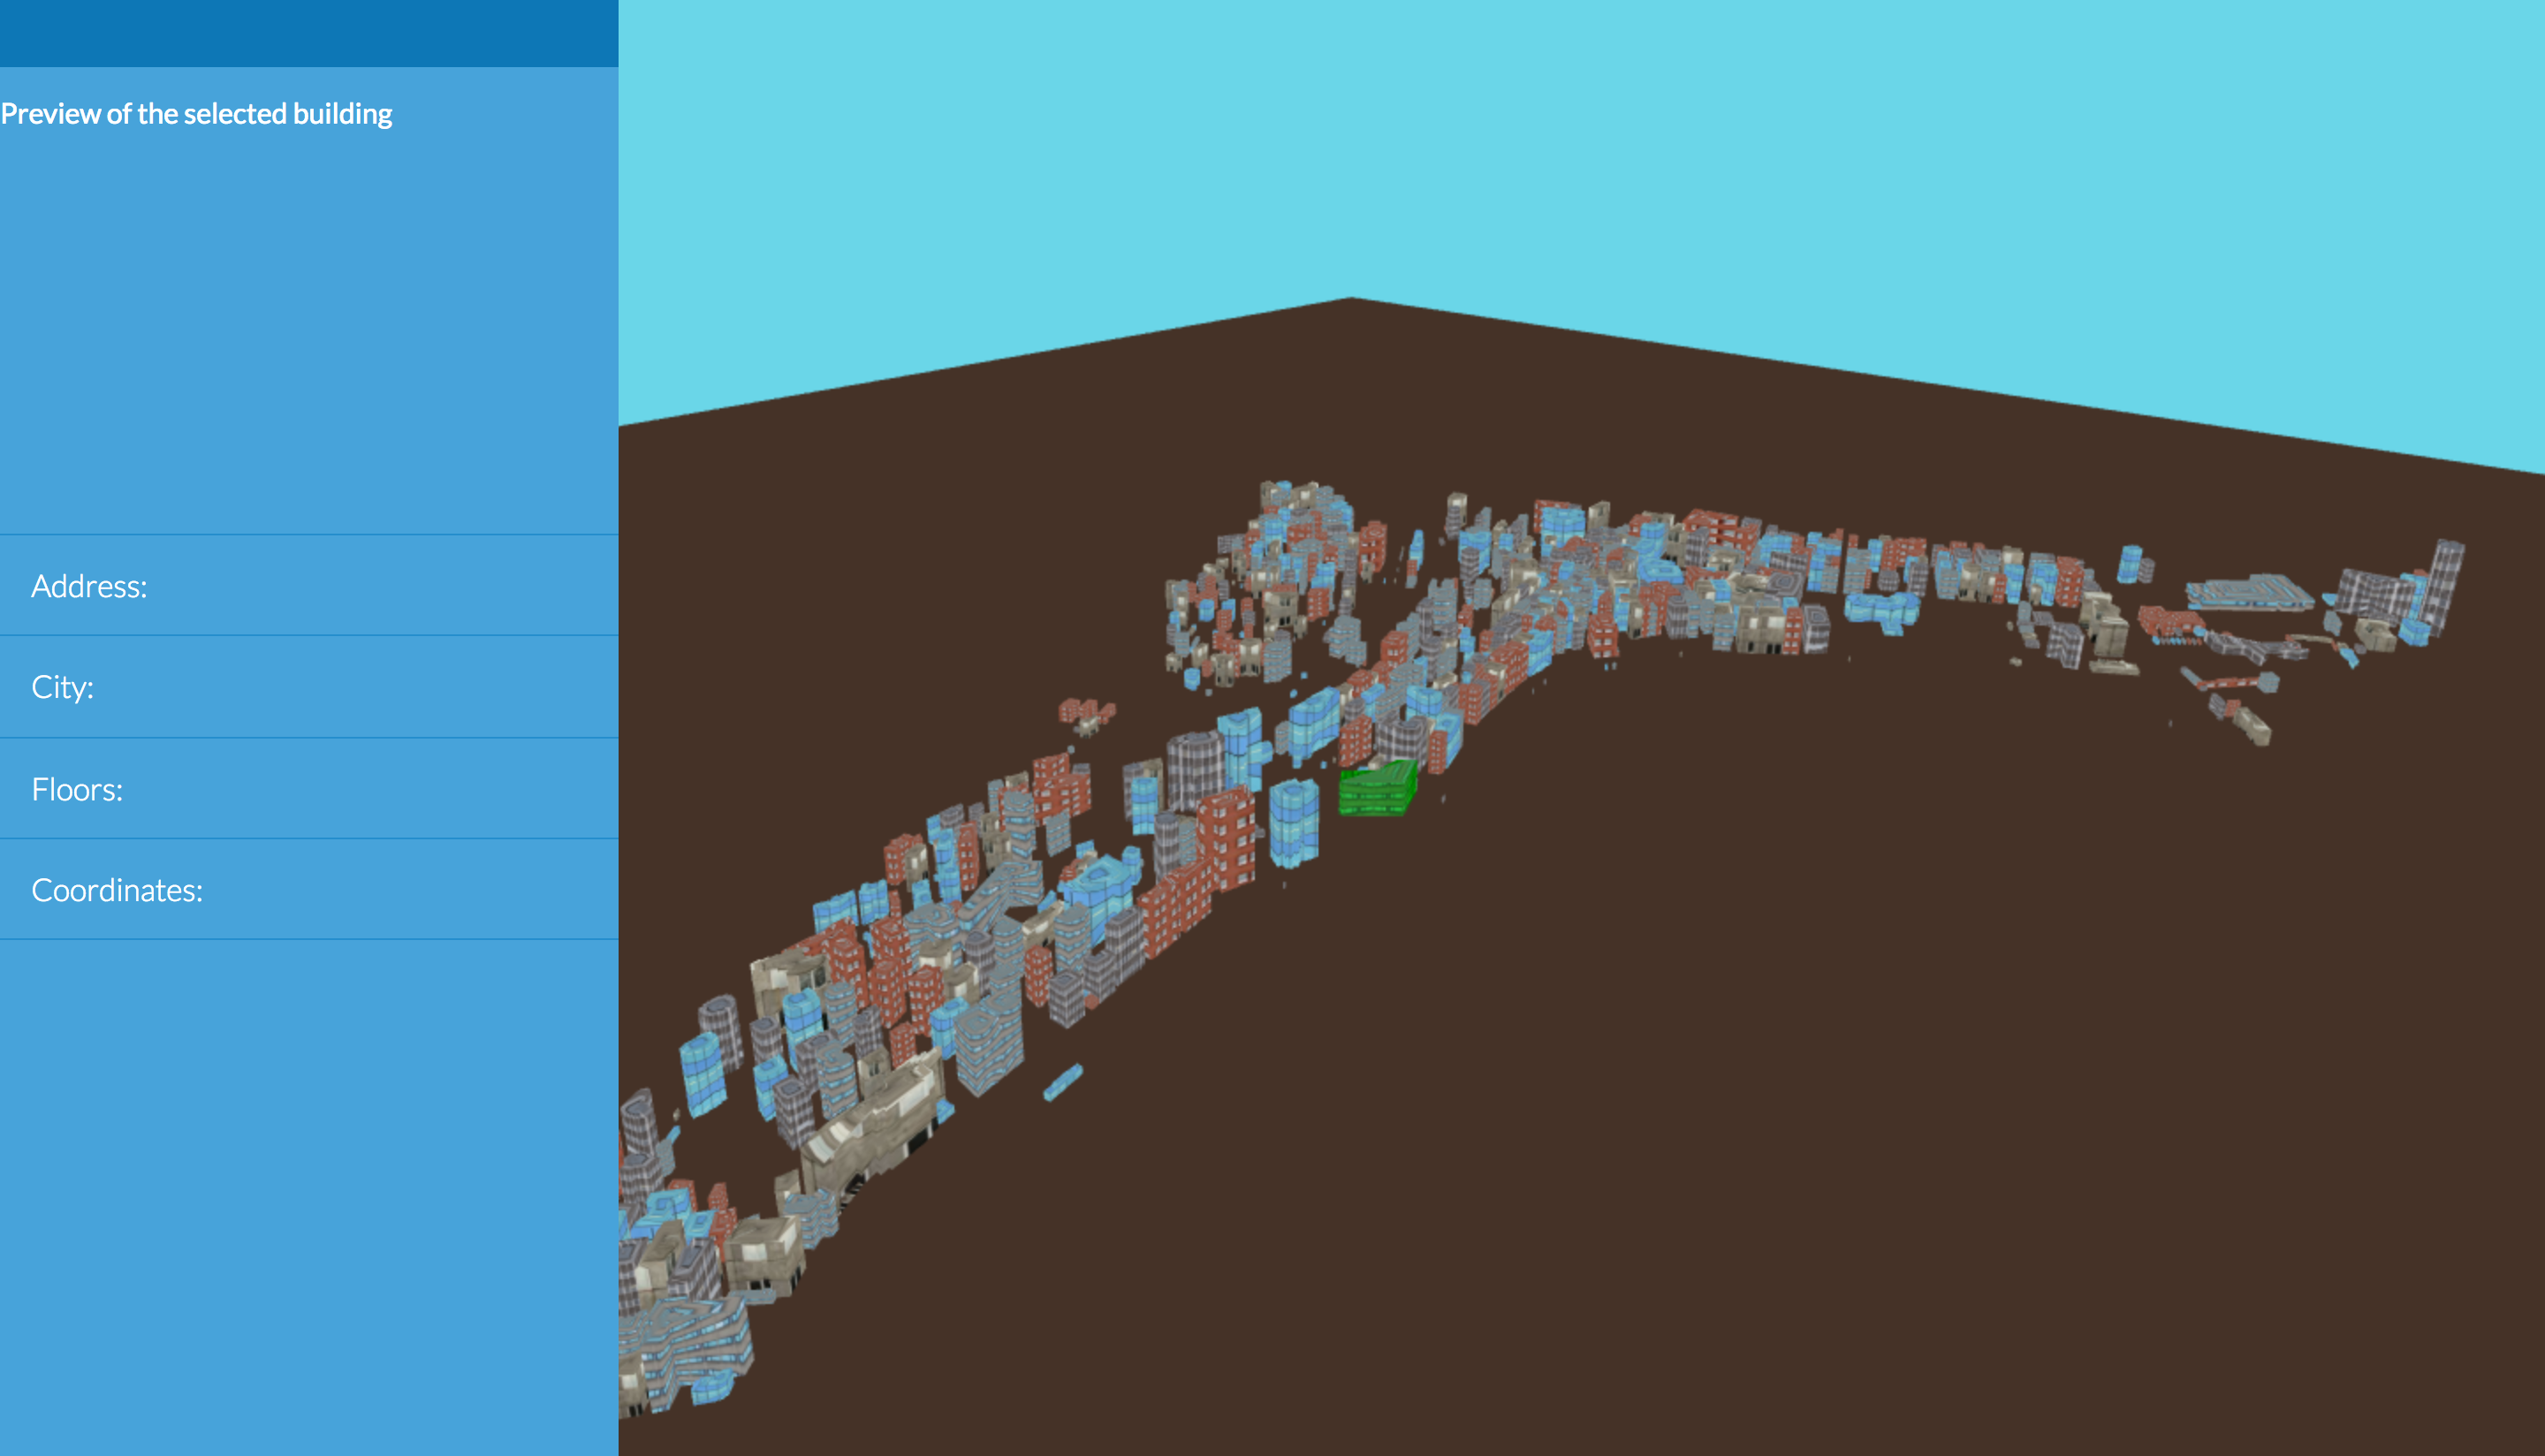
\includegraphics[width=0.8\textwidth]{chapter3/images/babylonJS}
\caption{The first attempt of city visualization using BabilonJS}
\label{fig:babilonJS}
\end{figure}
As long as the buildings showed in the scene where under $\sim 2000$, the browser was very fast in rendering during the loading of the page and the movement of the camera was smooth.\\
The main problems that make the idea to use BabylonJS discarded, were has been basically two:
\begin{itemize}
	\item The buildings to be rendered were far above the mentioned threshold, the rendering would take more than 30 seconds.
	\item BabylonJS provides no basis to start from: the initial scene is completely empty and, as it is possible to see in the image above, buildings lay on a plane. That represented a serious problem since the visualization of the city was planned to be shown in a way that would be as realistic as possible.
\end{itemize}
A solution to the last problem would have been using the Google Elevation API. This service, given a pair of coordinates (i.e., latitude and longitude), returns the exact altitude of that point.\\

Unfortunately, the API system of Google provides just 2,500 free requests per day. In the case of Lugano, that extends its territory for more that $25km^2$, considering one request for meter it would have been taken more than 10 days to get the entire terrain structure (for the entire city of Rome, that spans almost $46km^2$, the days taken would have been more than 20).\\

Nonetheless, this would have made the rendering slower since, in addition to the visualization of the buildings, also a rendering of the terrain (i.e., lakes, mountains and rivers) would have taken place.\\
Therefore, this lack of both Google--API--requests and good performances, lead the idea to use BabylonJS to be discarded. Later, during the development of \applicationName, Babilon.js was reintroduced just to render the building model in the Info--Box about the selected building. 
\subsubsection{The final version: Cesium.js}
As stated above, the Cesium Framework was finally used to build the client--side of the application.\\
Cesium, on the contrary, provides a ready--to--use virtual globe in which it is possible to directly create shapes and polygons using coordinates in WGS as points. As stated before, Cesium is provided with a full documentation about its APIs in which it is possible to control and modify every aspect of this framework: from the provided menu to the drawing of complex polygons of the surface.\\

In addition to this, on Cesium it is also possible to select a particular terrain provider (in the case of \applicationName, we used the STK), which allows to visualize global high--resolution terrains and represent mountains, valleys and other terrain features. In addition, an API on Cesium is provided in which, given a terrain provider and a point on the map, it is possible to know the elevation of that point without a maximum limit of requests. That solved the problem presented above that was the limited number of requests provided by Google in order to get the elevation of a coordinate.\\

In order to render the buildings on the map, the polygonGeometry API has been used: among all the attributes that this object takes (i.e., type of shadow, color, definition, etc\dots), it also takes an array of coordinates. These are the coordinates of the point useful to draw the geometry. Therefore, in order to draw the entire city of Lugano on the startup of the application, it makes a request to the server in order to get the coordinates (in WGS) of the buildings in the desired city, then they are rendered one at a time on the map. This operation done in Cesium is quite performing since it takes $\sim 5$ seconds to render the entire city of Lugano and then, the operation of rotating and moving the camera is very smooth (on the contrary of what was achieved using Babylon.js).\\

All the issues encountered with the use of Babylon.js were solved by using the Cesium Framework. That is why we decided that \applicationName\ has to rest on this techonlogy.   
\subsubsection{Provided Interface}
\applicationName\ aims to create interactive 3D cities representations accessible by everyone. In order to have interactions that may suggest interest in users, it is required to have an user--friendly system which allows interactions with the entities in the city. In order to achieve this feature in the most flexible way, a tab based interface is at disposal of the user. The proposed interface is composed as follows:
\begin{itemize}
	\item An {\bf Info--Box} is shown whenever a building is selected. All the available information about it are displayed such as: street name, civic number, membership suburb, number of floors, purpose of the building, EGID value, perimeter length, area of the building and Percentace of Primary and Secondary Houses. On top of the Info--Box is also possible to interact with a stand--alone model of the building rendered using Babylon.js.
	\item A {\bf sidebar} is at user's disposal and it is divided into the following subsections:
	\begin{itemize}
		\item The {\bf Visualize} Tab let the user: {\bf add elements} to the city like the geolocalization and the position of the cameras distributed around the city, {\bf color} the city by height or by suburb and decide to {\bf show some suburbs} rather than others.
		\item The {\bf Query City} Tab is the core of the interaction between the user and the city visualization. It is possible to create a completely personalized query, selecting which field to search and which value should be searched. This part will be better explained later in this report.
		\item The {\bf Query History} Tab contains the list of all the queries executed during the session, showing the number of results for every different query.
		\item The {\bf Credits} Tab just contains information about who worked on this project and what technologies were used for the 3D--visualization.
	\end{itemize}
\end{itemize}
\subsubsection{Query Builder}
The client side, takes advantage of the great flexibility given by the APIs created on the server--side and explained above. They are very useful in order to visualize on the city, results of the query executed visually on the sidebar.\\
Once the user has clicked on the {\bf Query City} tab, the interface shown will be the one on Figure \ref{fig:query_city_tab}.\\ 
\begin{figure}[H]
\centering
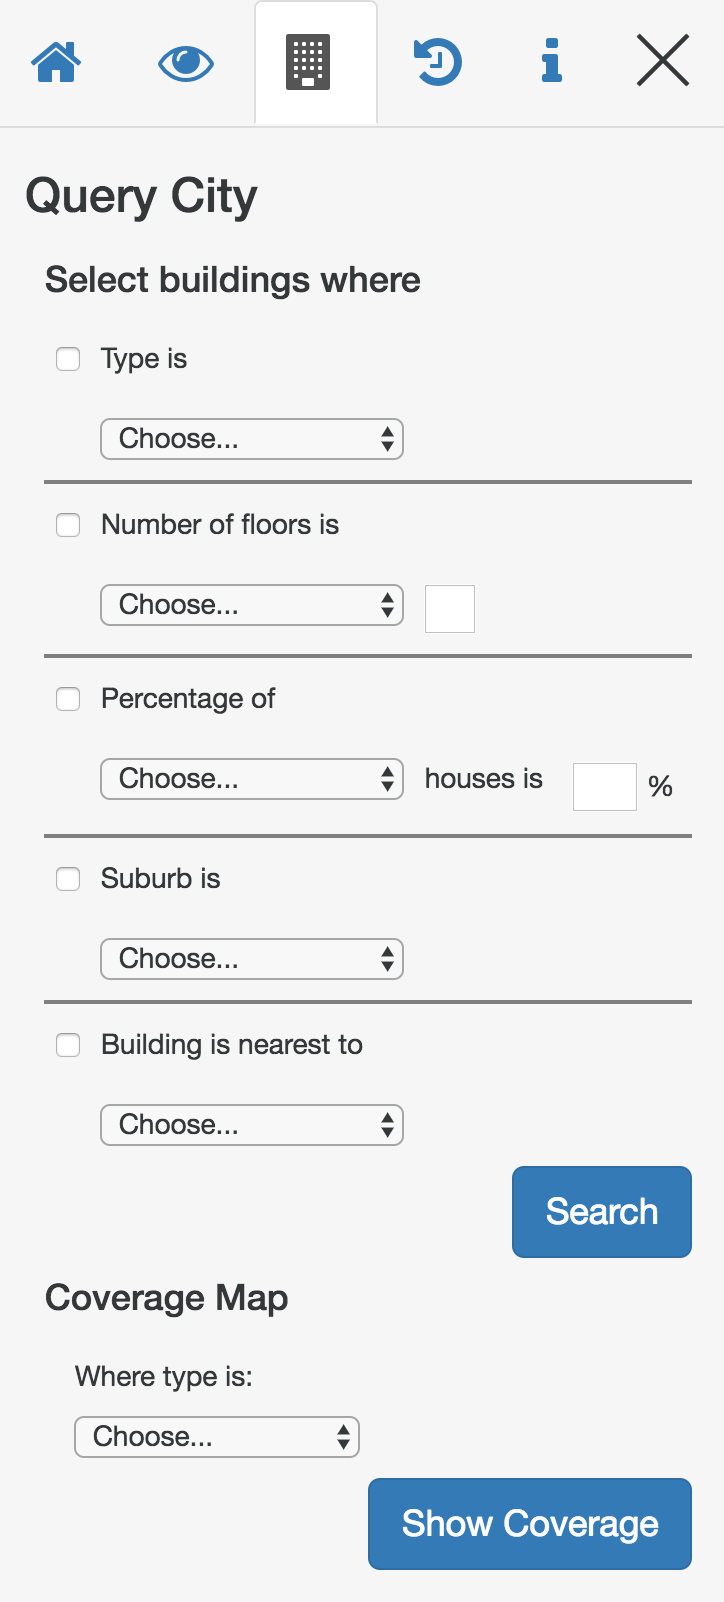
\includegraphics[width=0.35\textwidth]{chapter3/images/query_city_tab}
\caption{The Query City Tab}
\label{fig:query_city_tab}
\end{figure}
On the {\bf Select Buildings} subsection, it is possible to select, row by row, which constraint to add to the final query. The user would only have to check the checkbox and set a value for that specific field. Of course, it is also possible to select multiple rows in order to do more restrictive queries. The buildings that match the executed query, will be highlighted with a different color.\\

On the {\bf Coverage Map} subsection, it is instead possible to visualize on the map the coverage of certain buildings considered hotspots of the city. The result of this kind of query will occur colouring the hotspot (or hotspots if many of the same type) in red, the neighbour buildings will be coloured with an interpolation of colours from lime green to with depending on their distance from the hotspot.\\

Both kind of queries, will be better explained and enhanced with visual examples in the chapter called ``Use cases'', later in this report. 
